\documentclass[11pt, twocolumn]{article}
\usepackage[a4paper, hmargin={2.8cm, 2.8cm}, vmargin={2.5cm, 2.5cm}]{geometry}
%\usepackage[T1]{fontenc}
\usepackage[utf8]{inputenc}
\usepackage{eso-pic} % \AddToShipoutPicture
\usepackage{graphicx} % \includegraphics
\usepackage[english]{babel}
\usepackage{multicol}
\usepackage{amssymb}
\usepackage{amsmath}
\usepackage{fancyhdr}
\usepackage{fancyvrb}
\usepackage{geometry}
\usepackage{listings}
\usepackage{mips}
\usepackage[hyphens]{url}
\usepackage{breakurl}
\usepackage{cite}
\usepackage{color}
\usepackage{array}
\usepackage{multicol}
\usepackage[toc,page]{appendix}
\usepackage{cleveref}
\usepackage[breaklinks=true]{hyperref}
%\usepackage[breaklinks=true,pdfborder={0 0 0},bookmarksopen]{hyperref}
\usepackage{float}
\usepackage{xcolor,colortbl}
\usepackage{soul}
\usepackage{pdfpages}
\usepackage{multirow}
\usepackage[font={small,it},skip=0pt]{caption}
\captionsetup[figure]{font={small,it},skip=2pt}
\usepackage{tablefootnote}
\usepackage{footnote}
\usepackage{subcaption}
\usepackage{lipsum}


\makesavenoteenv{tabular}

% More subsubsub sections

\iffalse
\usepackage{titlesec}
\setcounter{secnumdepth}{4}
\titleformat{\paragraph}
{\normalfont\normalsize\bfseries}{\theparagraph}{1em}{}
\titlespacing*{\paragraph}
{0pt}{3.25ex plus 1ex minus .2ex}{1.5ex plus .2ex}
\fi

\errorcontextlines 10000


\raggedbottom


\newcommand\floor[1]{\lfloor#1\rfloor}

\definecolor{tablegreen}{rgb}{0.609375, 0.8828125, 0.3515625}
\definecolor{tableyellow}{rgb}{0.9921875, 0.859375, 0.2734375}
\definecolor{dkgreen}{rgb}{0,0.6,0}
\definecolor{gray}{rgb}{0.5,0.5,0.5}
\definecolor{mauve}{rgb}{0.58,0,0.82}


\newcolumntype{C}[1]{>{\centering\let\newline\\\arraybackslash\hspace{0pt}}m{#1}}
\setlength{\columnsep}{1cm}


\lstset{ %
	language=[mips]Assembler,       	% (small) MIPS assembly
		basicstyle=\footnotesize,       % the size of the fonts that are used for the code
		numberstyle=\tiny\color{gray},  % the style that is used for the line-numbers
		stepnumber=1,                   % the step between two line-numbers. If it's 1, each line
		% will be numbered
		numbersep=5pt,                  % how far the line-numbers are from the code
		backgroundcolor=\color{white},  % choose the background color. You must add \usepackage{color}
		showspaces=false,               % show spaces adding particular underscores
		showstringspaces=false,         % underline spaces within strings
		showtabs=false,                 % show tabs within strings adding particular underscores
		frame=single,                   % adds a frame around the code
		rulecolor=\color{black},        % if not set, the frame-color may be changed on line-breaks within not-black text (e.g. commens (green here))
		tabsize=4,                      % sets default tabsize to 2 spaces
		captionpos=b,                   % sets the caption-position to bottom
		breaklines=true,                % sets automatic line breaking
		breakatwhitespace=false,        % sets if automatic breaks should only happen at whitespace
		title=\lstname,                 % show the filename of files included with \lstinputlisting;
		keywordstyle=\color{blue},          % keyword style
		commentstyle=\color{dkgreen},       % comment style
		stringstyle=\color{mauve},         % string literal style
		escapeinside={\%*}{*)},            % if you want to add a comment within your code
		morekeywords={*,...}               % if you want to add more keywords to the set
}


\lstdefinestyle{customc}{
	belowcaptionskip=1\baselineskip,
		breaklines=true,
		frame=L,
		xleftmargin=\parindent,
		language=C,
		showstringspaces=false,
		basicstyle=\footnotesize\ttfamily,
		keywordstyle=\bfseries\color{green!40!black},
		commentstyle=\itshape\color{purple!40!black},
		identifierstyle=\color{blue},
		stringstyle=\color{orange},
}





\definecolor{dkgreen}{rgb}{0,0.6,0}
\definecolor{gray}{rgb}{0.5,0.5,0.5}
\definecolor{mauve}{rgb}{0.58,0,0.82}

\newcommand{\pic}[3] {
	\begin{figure}[ht]
		\centering
		\includegraphics[width=#3\textwidth]{#1}
	\caption{#2}
	\label{fig:#1}
	\end{figure}
}


\newcommand{\picappendix}[3] {
	\begin{figure}[H]
		\centering
		\includegraphics[width=#3\textwidth]{#1}
	\caption{#2}
	\label{fig:#1}
	\end{figure}
}

\newcommand{\asmcode}[3] {
	% \begin{figure}[H]
		% \centering
		\begin{Verbatim}[fontsize=\scriptsize]
#3
		\end{Verbatim}
	\caption{#2}
	\label{fig:#1}
	% \end{figure}
}

\newcommand{\dpic}[5] {
	\begin{figure}[h]
		\centering
		\begin{subfigure}{#5\textwidth}
	\centering
		\includegraphics[width=.9\linewidth]{#1}
	\caption{#2}
	\label{fig:#1}
	\end{subfigure}%
		\begin{subfigure}{#5\textwidth}
	\centering
		\includegraphics[width=.9\linewidth]{#3}
	\caption{#4}
	\label{fig:#3}
	\end{subfigure}
	\end{figure}
}

\author{
	\Large{
		\begin{tabular}{C{4.5cm} C{4.5cm} C{4.5cm}}
		Jan Mezník \\
			\texttt{PZJ895}
		\end{tabular}
	}
	\vspace{12cm}
}

\title{
	\vspace{3cm}
	\huge{See KUDOS Run}\\
%	\Huge{Simulation of a MIPS machine} \\
		\vspace{0.5cm}
	\Large{A MIPS machine simulator}
}

\begin{document}


\onecolumn


%%%%% KU HEADER %%%%%%%%%%%%%%%%%%%%%%%
%% Change `ku-farve` to `nat-farve` to use SCIENCE's old colors or
%% `natbio-farve` to use SCIENCE's new colors and logo.
\AddToShipoutPicture*{\put(0,0){\includegraphics*[viewport=0 0 700 600]{include/ku-farve}}}
\AddToShipoutPicture*{\put(0,602){\includegraphics*[viewport=0 600 700 1600]{include/ku-farve}}}

%% Change `ku-en` to `nat-en` to use the `Faculty of Science` header
\AddToShipoutPicture*{\put(0,0){\includegraphics*{include/ku-en}}}


%\clearpage
\maketitle
\pagenumbering{roman}
\thispagestyle{empty}
\newpage
%%%%%%%%%%%%%%%%%%%%%%%%%%%%%%%%%%%%%%%

\begin{abstract}
\thispagestyle{empty}
TODO

\end{abstract}

\section*{Overview}
This report serves as documentation to the MIPS simulator, codename
\texttt{See KUDOS Run}, written as a part of a bachelor project at University
of Copenhagen. See KUDOS Run is a machine simulator, containing pipelined CPUs,
memory-management unit, IO-mapped devices as well as external devices.\\
The simulator and the version-controlled source-code is located at \url{https://github.com/JanmanX/MIPS-Simulator}.
\subsection*{Building the simulator}
After downloading the source, the simulator can be built using:
\begin{verbatim}
$ make
\end{verbatim}
The simulator should be built in the \texttt{./bin/} directory as \texttt{mips-sim}.\\
A few test-programs are supplied along the simulator. These must be compiled
using a cross-compiler. A shell-script installing the cross-compiler is supplied
along side the simulator:
\begin{verbatim}
$ ./tools/cross_compiler.sh
...
$ ./run_tests.sh
\end{verbatim}
\subsection*{Running the simulator}
The simulator has a variety of command-line options, which can all be listed
using the \texttt{-h} or \texttt{--help} flag.\\
Running the simulator can be as simple as only giving the program as the first
command-line argument:
\begin{verbatim}
$ ./bin/mips-sim tests/test_add_addiu.elf
$ echo $?
60
\end{verbatim}
To run a program with debugging enabled, the \texttt{-d} flag is supplied, which
will let the user step the instructions:
\begin{verbatim}
$ ./bin/mips-sim -d tests/test_add_addiu.elf
PC: 0x80010000
0x2408000A	ADDIU  rs = zero = 0x00000000,  rt = t0 = 0x00000000,  imm = 0x0000000A
> q
\end{verbatim}


\newpage

\section*{Preface}
\subsection*{Updated Problem Statement}
Is it possible to implement a pipelined MIPS simulator, with a memory-management
unit, memory-mapped IO, and full exception support, to fully support the
current version of KUDOS?

\subsection*{Target Audience and Prerequisites}
This report is intended for anyone interested in computer architecuture, with
the desire to expand the knowledge on the inner workings of MIPS32 processors.\\
The reader is expected to have either recently have taken a computer architecture course
or read \textit{Computer Organization And Design: The Hardware/Software Interface, 5th
edition, by David A. Petterson and John L. Hennessy}, particularly focusing on
the instruction pipelining within the processing unit.\\
Additionally, some fundamental understanding of computer hardware and related lingo is required,
as well as a basic understanding of programming languages and data-structures.

\subsection*{Downloading and building the simulator}
The simulator can be downloaded and built using:
\begin{verbatim}
$ git clone https://github.com/JanmanX/MIPS-Simulator.git
$ cd MIPS-Simulator/
$ make
\end{verbatim}
The simulator should be built in the \texttt{./bin/} directory as \texttt{mips-sim}.\\
A few test-programs are supplied along the simulator. These must be compiled
using a cross-compiler. A shell-script installing the cross-compiler is supplied
along side the simulator:
\begin{verbatim}
$ ./tools/cross_compiler.sh
...
$ ./run_tests.sh
\end{verbatim}
\subsection*{Running the simulator}
The simulator has a variety of command-line options, which can all be listed
using the \texttt{-h} or \texttt{--help} flag.\\
Running the simulator can be as simple as only giving the program path as the first
command-line argument:
\begin{verbatim}
$ ./bin/mips-sim tests/test_add_addiu.elf
$ echo $?
60
\end{verbatim}
To run a program with debugging enabled, the \texttt{-d} flag is supplied, which
will let the user step the instructions:
\begin{verbatim}
$ ./bin/mips-sim -d tests/test_add_addiu.elf
PC: 0x80010000
0x2408000A	ADDIU  rs = zero = 0x00000000,  rt = t0 = 0x00000000,  imm = 0x0000000A
> q
\end{verbatim}


\newpage

\twocolumn

%\thispagestyle{empty}
\tableofcontents

\onecolumn
\newpage
\twocolumn

\clearpage
\pagenumbering{arabic}
\setcounter{page}{1}

\markboth{Name}{Report}
\noindent
%\underline{\textbf{Category}}\\
%Hardware emulation\\\\
%\underline{\textbf{Keywords}}\\
%Copenhagen, university, computer, science, simulation, MIPS

\section{Introduction}
This report describes the development of a MIPS simulator, intended to support
the operating system KUDOS. The simulator will be written in C, and will
support the most important processor features and I/O devices, required to run
KUDOS, such as the translation lookaside
buffer (TLB), memory management unit (MMU), user and kernel CPU modes,
multiple cores (SMP), and I/O device emulation. \\


\subsection{Motivation}
KUDOS is a small operating system skeleton intended to be used by students
attending operating system project courses at university of Copenhagen.
It is used to explore operating system concepts by extending and improving on
existing system.
Initially, KUDOS targets the MIPS32 architecture, which leverages on the
advantages of a
reduced instruction set computing --- RISC.\\
To ease the development and debugging of KUDOS, it is desireable to run the
operating system
in a simulated machine. This enables the students and other developers to
better inspect the state of the machine, as well as making up
for the difference in the hardware of the host machine.

\subsection{A simulator}
A simulator is a program or a machine, that models some key characteristics
and functions of a given target.  The purpose of a
simulator is to be able to look inside the simulation and inspect the properties
and behaviours, that would otherwise only be seen in the real target.
A possible by-product of a simulator is that the simulation model will emulate
the target and its behaviour, practically immitating the target.\\
An emulator, on the other side, is intended to only mimick the behaviour of
a target on the outside, not correctly reflecting the internal state of the target.
Emulators are often used as a substitute for the real targets.
The difference between emulation and simulation is therefore, that unlike simulating a system,
an emulator only imitates the outward behaviour of its target, and it is hard
to predict how the target would act internally.\\
For example, mobile developers often use an emulator to test their
applications.
Instead of having thousands of real smartphones, they can simply emulate\footnote{
To be precise, they are emulating the hardware devices, but the applications they
are testing, are being simulated.}
the devices on their computers, saving both time and money.\\
A common use of a simulator is in the aircraft business, where flight-simulators
are being used for both pilot training, engineering, design, and many other
purposes. While it gives a very good insight on how a simulated airplane might
react in given situations, it does not actually move the users from one point
to another.\\
The purpose of our project is to write a program used at the Computer Systems
course at Copenhagen University, that can emulate KUDOS, while at the same
time, exposes the internal workings of the machine, for the students and
other participants to inspect and study.\\
Our target is therefore to simulate the academically important and relevant
parts, while others will be emulated.



\section{Background}
KUDOS is heavily based on the BUENOS operating system, originally developed at
Aalto University, Finland\cite{readthedocs:kudos}.\\
Although KUDOS has been extended for the x86 architecture, it mainly supports
MIPS32 architecture, just as its predecessor. The OS has been developed along
side a machine simulator YAMS (\textit{Yet Another Machine Simulator}), which
is used to run the operating system.\cite{readthedocs:kudos}


\subsection{KUDOS and YAMS}
BUENOS, and thus KUDOS, has been developed very closely with the YAMS simulator.
Since the intetion of the OS is to be used at operating system courses, it is
heavily dependant on the simulator, its interfaces, and its devices.\\
Despite being a very simple and basic simulation of a machine, it is still a
very realistic hardware interface.


\subsection{Analysis}
The KUDOS operating system is written to fully utilize the many of MIPS32 features,
which the students can research and extend.\\
To be able to run KUDOS correctly, the simulator must at least support the features
listed below:
\begin{itemize}
	\item \texttt{Translation Lookaside Buffer}\\
Most noteably, KUDOS lets the students research and extend the Translation
Lookaside Buffer (TLB), which is a cache used to translate virtual addresses\cite{COD5}.\\

	\item \texttt{TTY device}\\
A typewriter, more commonly known as a TTY is required, to be able to communicate
with the operating system. These devices are usually very basic, only being able
to transmit textual messages.

	\item \texttt{Shutdown device}\\
The operating system needs a way to cleanly shutdown. The simulator will setup
this device, and when required, will efficiently bring the system down.

	\item \texttt{Mapping of all memory segments}\\
KUDOS may be extended to fully utilize the entire main memory. As memory is
split into segments in MIPS32, it is essential for the simulator to be able to
handle this.

	\item \texttt{Bootstrapping mechanism}\\
KUDOS is shipped without a bootloader, relying on the simulator to correctly
load the OS and start it from an appropriate point.
\end{itemize}



\subsection{Design Goals}
For the simulator to work flawlessly with KUDOS, it will be heavily inspired by
the YAMS simulator. Since the OS is relying on the simulator, and vice versa,
we do not want to make any drastic changes to the simulator, as to avoid rewriting
parts of KUDOS. The main design goals of the simulator are:\\
\begin{itemize}
\item \textit{Avoid breaking compatibility}\\
For better integration of the simulator into the operating systems course, it is
undesireable to make such big design changes, that would need to be patched in
the OS as well. Even minor changes in KUDOS could break previously working
code, such as assignments and exercises.

\item \textit{Simplicity over performance}\\
The goal of the simulator is to seamlessly interface with the OS, while still
being simple to understand and research. KUDOS is a very simple OS, and YAMS is
by no means computationally intensive -- the host machine should have no problems
running both. Therefore, we want to focus on the readability rather than on the
performance.

\item \textit{Usability}\\
The simulator should be easy to use, stable, and flexible in regards of its
functionality.
Apart from running the OS and other simulated programs, the users should be able
to stop the running program, to inspect the state of the simulated machine.
\end{itemize}


\section{CPU Architectures}
At the heart of every computer lies the Central Processing Unit (CPU),
which is
an electronic circuit that carries out the basic arithmethic- and logic
calculation as well as process and redirect input and output to other devices
in the computer, using the shared busses.

Most modern CPUs are contained on a very small, yet packed intergrated circuit
chip, which can also house memory caches, multiple cores, and other processing
units.

The functionality of all processors is fundamentally the same. The processor
executes some primitive operation by fetching an instruction in the form of
binary signals, act upon the instruction and store the result in either
one of the its registers, or in the main memory.

A single instruction does very little, but a collection of instructions
make up
a program. In the very early computing days, computers were programmed in an
assembly language, which is simply human-readable instruction code. As the
computers grew more powerful, more complex and much faster, larger programs could be
executed. Because it is hard and time-consuming to write programs using
only the
assembly language, compilers are used to remove this complexity. A
compiler takes a high-level language, such as C, C++ or Java, and creates the
corresponding assembly language program for the specific architecture,
containing the instructions. This assembly language file is in turn assembled
or translated to binary, that the particular CPU can understand.

Besides hiding the complexity of the underlying architecture away from the
programmer, it can usually also compile programs to multiple architectures as
well as optimising the code to run faster.

\subsection{Instruction Set Architectures}
The instructions supported by a particular processor is determined by the
Instruction Set Architecture (ISA), which is the specification of how the CPU
works. An ISA determines the instructions
supported, the registers available, memory architecture, addressing modes as
well as handling of interrupts.

There exists many different types of ISAs, with both their advantages and
disadvantages. For example, some architectures have a very few instructions
and registers, which is very practical for small embedded devices,
whereas large
servers might make use of a large array of registers for complex computations.

Besides the current use of an architecture, designers must also take into
account its future uses and applications. As the world of computation is ever
growing and evolving at exponential rates, the architectures must be up to the
challenge of future computing. Introducing a completely new architecture to
the market is very troublesome, and causes a list of problems.
One of the main issues is that old software written for older architectures
will no longer work, and it requires to be either recompiled, rewritten,
or even emulated. One such example is the Intel Itanium (IA-64) architecture,
which had a very bad marked reception due to its lack of backwards
compatibility
with the x86 architecture. The emulation of the architecture on IA-64 yielded
suboptimal performance and ultimately lost to the AMD x86\_64, which in
turn was
compatible.\cite{anandtech:1854}

Indeed, there are a lot of factors to take into account when designing a new
architecture, and every decision has big implications on the future of the
whole ISA.

\subsection{MIPS Architecture}
The MIPS architecture (acronym for Microprocessor without Interlocked Pipeline
Stages) was first created in the early 1980s.\cite{imgtec:MIPS_Overview}
MIPS is a reduced instruction set architecture (RISC), developed by MIPS
technologies, to bring new levels of
performance and efficiency into the world of processing units. As an RISC
architecture, MIPS aims to implement only the most essential instructions, so
that they in return can get highly optimised. This is the based on the RISC
philosophy, that by implementing only the most common instructions, the
architects can simplify the design and speed up the crucial parts of the
instructions. This enables the processor to execute programs faster, but also
removes a lot of complexity of implementing large programs.

In contrast to RISC, complex instruction set architecture (CISC) aims
to reduce the number of instructions needed to execute a program by
implementing instructions packed with functionality. This means that a single
instruction in CISC can execute several operations at once, such as loading
from memory, arithmetic
and storing. While complex programs indeed execute faster on a CISC
architecture,
the burden of implementing efficient and maintainable code and compilers can
outweigh its advantages. \cite{Patterson:1980:CRI:641914.641917}

Besides the inspiration from RISC, MIPS has added its own design principles,
which are honored and used to question every change, implementation,
or design.
These are \cite{COD5}:
\begin{itemize}
	\item \textit{Design Principle 1:} Simplicity favors regularity.
	\item \textit{Design Principle 2:} Smaller is faster.
	\item \textit{Design Principle 3:} Good design demands good
	compromises.
	\item \textit{Design Principle 4:} Make common case fast.
\end{itemize}
These decisions withstood the trial by fire and proved, that honoring these
principles yields good design, easing implementation as well as simplifying
hardware.


\section{MIPS Core Processing Unit}
MIPS CPUs are pipelined, meaning that it implements a pipeline which
enables it
to execute different stages of multiple instructions at once. This gives the
processor a higher throughput that would otherwise be possible at a given
clock-rate. The processor has 31 general purpose (GP) registers, with
additional registers
per co-processing unit. Even the first models of the MIPS CPUs, such as the
MIPS R2000, had memory caches and a translation lookaside-buffer, which improves
the speed of the processor by reducing the number of main memory lookups.

\subsection{Registers}
MIPS contains multiple types of registers. The most common and most used
registers are the general-purpose registers (GP), which can be used for
practically anything by the programmer. Special registers are registers
implemented for cases where GP registers were either too small or otherwise
unsuitable for the purpose.\\
For additional functionality, the MIPS co-processor 0 also has its own set of
registers that, along with an operating system, bring many features to the
system.

\subsubsection{General Purpose Registers}
In MIPS, there are 32 general-purpose registers, all 32 bit wide. Although
they
can all theoretically be used however the programmer or assembler
wants\footnote{Except the 0'th (\$0) register, which can only hold the
value 0.}, there
are some conventions for the use of the registers.
\begin{center}
    \begin{tabular}{ | l | l | l | c |}
    \hline
	\textbf{Mnemonic\footnote{Textual mnemonic used in the assembly language}}%
		 & \textbf{\#} & \textbf{Use} \\ \hline \hline
	\texttt{\$zero}		& 0	& Constant Value 0 \\ \hline
	\texttt{\$at}		& 1	& Reserved Temporary \\ \hline
	\texttt{\$v0-\$v1}	& 2-3	& Function Results \\ \hline
	\texttt{\$a0-\$a3}	& 4-7	& Function Arguments \\ \hline
	\texttt{\$t0-\$t7}	& 8-15	& Temporaries  \\ \hline
	\texttt{\$s0-\$s7}	& 16-23 & Saved Temporaries \\ \hline
	\texttt{\$t8-\$t9}	& 24-25 & Temporaries \\ \hline
	\texttt{\$k0-\$k1}	& 26-27 & Reserved for OS \\ \hline
	\texttt{\$gp}		& 28	& Global Pointer \\ \hline
	\texttt{\$sp}		& 29	& Stack Pointer \\ \hline
	\texttt{\$fp}		& 30	& Frame Pointer \\ \hline
	\texttt{\$ra}		& 31	& Return Address \\ \hline
    \end{tabular}
\end{center}

\subsubsection{Special Registers}
The special registers in MIPS cannot directly be accessed from the program.
Rather, they are modified by different instructions.
\begin{center}
    \begin{tabular}{ | l | l | l | c |}
    \hline
	\textbf{Name} & \textbf{\#} & \textbf{Use} \\ \hline \hline
	\texttt{HI}		& -	& Hi-word of 64bit value \\ \hline
	\texttt{LO}		& -	& Lo-word of 64bit value \\ \hline
	\texttt{\$PC}		& -	& Program Counter \\ \hline
    \end{tabular}
\end{center}
\texttt{HI} and \texttt{LO} registers are used to contain the result of a
multiplication or division, which, using 2 32bit registers, can end with a
64bit result.\\
The PC register is pretty self-explanatory, as it simply points the current
location in the program (or "counts" the instructions). On other
architectures,
this register is better known as the Instruction Pointer (IP).

\subsubsection{Co-processor 0 registers}
Registers in co-processor 0 are mainly used by the system, to provide
additional features. The co-processor can have 32 registers, but only few of
them are used consistently. Many of the empty registers are also defined
by the
manufacturer of the processor.
\begin{center}
    \begin{tabular}{ | l | l | l | c |}
    \hline
	\textbf{Name} & \textbf{\#} & \textbf{Use} \\ \hline \hline
	\texttt{index}		& -	& TLB entry index\\ \hline
	\texttt{random}		& -	& TLB random access register \\ \hline
	\texttt{entrylo}	& -	& Low order current TLB entry \\
	\hline
	\texttt{context}	& -	& Page-Table lookup addr. \\ \hline
	\texttt{vaddr}		& -	& Virtual address of exceptions
	\\ \hline
	\texttt{entryhi}	& -	& High order current TLB entry\\
	\hline
	\texttt{status}		& -	& Processor status \\ \hline
	\texttt{cause}		& -	& Exception cause \\ \hline
	\texttt{epc}		& -	& PC when exception occured \\ \hline
    \end{tabular}
\end{center}
The \texttt{status} register is a bit-field of flags used to signal the
current
state of the processor. It is similar to the \texttt{EFLAGS} register on
x86 architectures.

The rest of the registers will be discussed in depth in the SMP chapter.


\subsection{Instructions}
Each instruction in MIPS is 32-bit long, aligned to word. This simplifies the
instruction fetching, decoding, as well as disassembly of the program,
for both
the processor as well as the programmer.

In MIPS, the instructions have 3 basic formats:
\begin{figure}[H]
\centering
\subfigure[R-Format]{%
	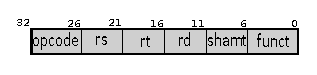
\includegraphics{cpu_architecture/r_format.eps}
	\label{fig:instruction_r_format}}
\subfigure[I-Format]{%
	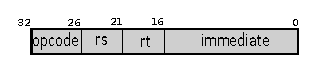
\includegraphics{cpu_architecture/i_format.eps}
	\label{fig:instruction_i_format}}
\subfigure[J-Format]{%
	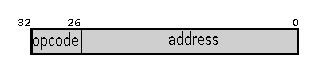
\includegraphics{cpu_architecture/j_format.eps}
	\label{fig:instruction_j_format}}
\label{fig:instruction_formats}
\end{figure}

It is clear that, as they have common fields, mainly the opcode field,
they are
easily distinguishable.\\
The R-format instructions are mainly used when all the data being processed is
located in the registers. That includes adding between registers, binary
operations on values in registers as well as jumping to an address located in
a register.\\\\
The I-format instructions can operate on both data from registers and
immediate
values encoded directly in the instruction (thus the 16-bit immediate field).
I-format instruction share a lot of common operations with the R-format, where
one of the operands is the immediate.\\\\
J-format instructions are used solely for jumping instructions, thus the large
address field. As it only has 26 bits to address an 32 byte memory location, it
shifts the whole value twice to the left, as to align the value in words. The
upper 4 bits are retrieved from PC. In practise, this is enough to jump to any
address in the program.

\subsection{Arithmetic Logic Unit}
Without any extension co-processing unit, the Arithmentic Logic Unit (ALU) in
MIPS32 only supports operations on integers. \\
The ALU supports basic mathematical operations such as adding (\texttt{add}),
subtracting (\texttt{sub}), as well as logical shifting to both left and right
(\texttt{sll, srl}), which also can be used to division or multiplication by
even numbers.

All bitwise logical operators \texttt{and, or, and nor} are implemented Using
these, which additional missing logical operations can be created, such as
\texttt{nand} and \texttt{not}.\\
Since both the operand and destination registers are 32 bit wide, an overflow
in the result might occur - that is, the result is larger than what a 32 bit
register can hold.
In that situation, an exception is raised in the processor, and code to recover
from this error is run\cite{COD5}. This will be explained in later sections.


\subsection{Load and Store}
MIPS is a "load/store" architecture, where memory is only accessed by specific
load and store instructions \cite{flynn1995computer}. This design is a very
common for RISC architectures, as it greatly simplifies the pipeline stages and
clock timings. In contrast, CISC architectures have many instructions that can
do operations on both memory and registers at the same time. For example, on
the x86\_64 architecture, the
\texttt{MOVSW} instruction reads from a memory location pointed to by register
SI, stores it in memory location DI, and at last, increments (or
decrements\footnote{This is determined by the direction flag, which determines
whether the CPU reads memory from top to bottom or in reverse.})
both registers\cite{intelmanual}. This adds additional stall and hazard logic to
the processor, and makes it is hard for the CPU to determine how many
clock-ticks the instruction will take.\\\\
MIPS32 uses \texttt{lw} for loading a word from the main memory into the register,
and a \texttt{sw}, which stores the value from register into the specified
memory location. In reality, MIPS32 also has \texttt{LH}, \texttt{LB} and
their store counterparts \texttt{SH} \texttt{SB}, which operate on half-word
and byte sized loads and stores. However, for performance reasons, the main
memory always reads a word (4 bytes), and so, the desired size is computed in
the CPU.



\subsection{Jumping and Branching}
To be turing complete, the processor needs to be able to do conditional jumps
to other memory locations. This is done with the jumping instructions: jump
(\texttt{j}), jump-register (\texttt{jr}) and jump-and-link (\texttt{jal}). The
conditional jumps are: branch-equal (\texttt{beq}) and branch-not-equal
(\texttt{bne}).\\
On the bare-metal level of the processor, these instructions simply modify the
value of the Program Counter register, which is otherwise inaccessible from
assembly.

\subsection{Interrupts}
Interrupts is a special way to control what the CPU. It actively "interrupts"
the CPU from its current job, and makes it execute a special function,
specified by an interrupt number. There usually 3 types of interrupts\cite{osdev:interrupts}:
\begin{itemize}
	\item Exceptions\\
	Exceptions occur in software, usually when an error has occurred that
	needs attention from the kernel. This is usually caused by reading from
	illegal memory addresses or when arithmetic overflow occurs.

	\item Hardware Interrupt\\
Hardware interrupts are initiated from hardware devices, such as a
mouse or a keyboard. When a user presses a key or moves the mouse, the hardware
devices send a signal to the CPU that something has happened that needs
attention from the kernel.

	\item System Call (syscall)\\
	Syscalls are usually used by programs, when they need attention from
the kernel. An operating system and the underlying kernel will usually expose
an interface with a whole set of functions, that the program can access by
syscalls. This can be everything from reporting termination of a program to
writing data to the disk.
\end{itemize}

The action that the CPU has to perform is determined by an interrupt vector
table. For each interrupt vector, there is specific code to be executed.
Because the interrupt vector table is limited in size, operating systems, such
as Linux, use a single interrupt vector number 0x80. Additional arguments for
further determination of the service are passed in service number, which is
stored in the general purpose registers, and if needed, in the stack.\\
System call handling is made somewhat easier in MIPS. Whereas in x86\_64, you
have to set the appropriate system-calls arguments and then do an interrupt on
the correct vector, MIPS has a dedicated system-call instruction
\texttt{syscall}. The operating system can choose however the arguments are
passed, but usually, the service number is stored in \texttt{\$v0}, and the
arguments in \texttt{\$a0-\$a3}\cite{COD5}.



% MIPS supports up
%to 4 coprocessors (COP), with each COP extending on the basic functionality. The
%only required co-processor is COP0, which is the System Control Coprocessor.
%Other co-processors usually available, but not required, are the floating-point operation
%coprocessor COP1 (FPU), the user defined COP2.






\section{Privilege levels}
To tighten the security, prevent software faults, and to protect the user from
malware, most modern hardware support mechanisms to detect the malicious behaviour
and act accordingly.\\
Most computer operating systems have access to different resources, ranging from
widely available devices to critical subsystems. To prevent malicious
program or defective code to take over the machine, it is desireable to keep
track of the execution, limiting the access to certain systems.\\
While limited checks can be done by the operating system, it is much more
secure and efficient to let the hardware, in our case, the CPU, to keep track
of each action, stopping on any suspicious activity.\\
This protection mechanism is often called "Protection rings", where the privilege
of a program is determined by the position on a privilege ring --- the inner ring 0
often called "kernel" for being the most privileged, to the outtermost ring,
often used by user applications. Depending on the architecture, the protection
ring can have multiple layers.

\subsection{Kernel and User mode}
MIPS supports only 2 privilege levels\footnote{All MIPS processors after R4000 model have a
third \textit{supervisor} mode. This mode is mostly ignored by operating systems,
and will not be discussed or used here.\cite{see_mips_run}}, called the kernel and user mode,
distinguished by a bit in the status register. While competing processors support
more levels, such as x86 supporting 4\cite{intelmanual} levels and ARM supporting 3\cite{arm:migrating_5_7},
they are very rarely used in practice.\\
The usage of the two privilege modes is very intuitive --- kernel mode is used
by the operating system and its kernel, while user mode is used for user applictions
only.\\
There are multiple functionalities these modes control, ranging from memory access
to instruction access.

\subsubsection{Memory and IO access}
In user mode, a MIPS32 processor can only access the bottom half of the memory
space, that is, the first 2GB. For addresses over, the processor will check
the top bit of the address and the privilege level, restricting non-kernel mode.
However, if the processor has a memory-management unit (discussed in section \ref{sec:mmu}),
the operating itself can control the process access to the memory, preventing
any reads and writes to restricted areas.

\subsubsection{kernel instructions}
Some instructions are restricted to the kernel mode only, because they can have
system-wide implications. These instructions are called privileged
instruction, and consist mainly of instructions that move data to and from
co-processor 0, such as \texttt{mfc0} and \texttt{mtc0}.


\subsection{Implementation}
In the simulator, there is no separate need for a module checking the
privileges of the executing process. The privilege checks are done every time
the processor executes an operation with special need, by inspecting the 3rd
and 4th bit of the status register, called the KSU\footnote{In COD5, the lower
bit of this field is called \texttt{UM} for User-Mode\cite{COD5}}.\\
If the process does not satisfy the privilege check, an appropriate exception
returned from originating function. This exception is then handled in the WB
stage, described in section \ref{sec:exceptions}.\\
It is to be noted that when handling exceptions, if the EXL flag is on, the
processor is automatically assumed to be in kernel-mode\cite{see_mips_run}.


\section{Pipeline}
CPU speeds are usually measured by timing the execution time of programs. Since
a computer program is just a collection instructions, the speed of the CPU is
determined by how fast it can process each instruction.
Every CPU has a clock, which ticks at a given rate. For every tick, a new
instruction is executed. This clock ensures that all instructions "flow" through
the processor without problems, and that the electrical components, such as the
ALU or the control-unit, can manage to carry out their tasks in that time.
Naturally, electrical engineers have pushed the limits of the circuits to manage
the highest clock rate. The clock rate of the very first processors was measured
in hertz and kiloHertz (kHz), but most modern desktop CPUs reach in multiple
GigaHertz (GHz)\cite{wiki:clock_rate}. However, even with those speeds, the
demand for faster processing units is ever-growing, and other techniques to speed-up
the execution are used.\\
One of those techniques is pipelining, which separates the circuit into multiple
stages, much like the assembly lines in factories. In such factories, workers
have their own station at the assembly line, do a specific task repeatedly, and
forward it down the line. This greatly increases the throughput of a factory and
decreases the labor need.
In MIPS, this idea is implemented by separating the processor into 5 stages\cite{COD5}:
\begin{itemize}
	\item Instruction Fetch (IF)
Fetches the next instruction.

	\item Instruction Decode (ID)
Reads the instruction, sets the appropriate control flags, reads the relevant
registers and sends the data to the next stage.

	\item Execute
Executes the instruction. This is typically done by the ALU with the appropriate
operation supplied.

	\item Memory Access
All operations on memory happen here. This stage either loads a memory address
or stores a value at an appropriate address.

	\item Write Back
Writes the results to the CPU registers.
\end{itemize}
Each of these stages will naturally use less time than all of them combined, and
since the clock is shared in all stages, it is set to the slowest stage in the
pipeline.\\
Not only do we have faster tick rate on our clock, but we are also able to
perform multiple operations concurrently. Figures \ref{fig:single_cycle_time}
and \ref{fig:pipeline_time} show the timing of each instruction, and how
pipelining might improve the whole process.
\begin{figure}[H]
        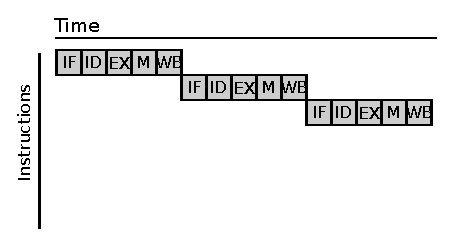
\includegraphics{pipeline/single_cycle.eps}
        \label{fig:single_cycle_time}
\end{figure}
\begin{figure}[H]
        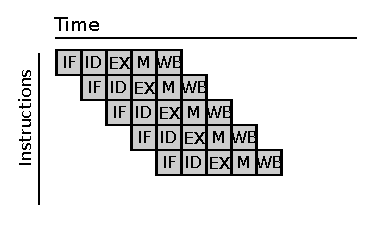
\includegraphics{pipeline/pipeline.eps}
        \label{fig:pipeline_time}
\end{figure}


\subsection{Design of the MIPS32 Pipeline}
The advantages of a pipelined design does not come without a price. Although
the single-cycle implementation of the processor is very similar to the
pipelined approach, it has its fair sets of challenges. The main problem with
executing instructions concurrently is that the instructions will often rely on
the result of the previous instructions. These situations are referred to as
hazards.

\subsubsection{Data Hazard}
Data hazards mainly occur when an instruction cannot continue, because it must
wait for the result from an earlier instruction. Suppose a program wants to
calculate the sum of 4 integers:
$$A = A + B + C + D$$
In MIPS32 assembly, this would be written as:
\begin{lstlisting}
# t0 = A, t1 = B, t2 = C, t3 = D
add $s0, $t0, $t1 	# s0 = A + B
add $s1, $t2, $t3	# s1 = C + D
add $v0, $s0, $s1
\end{lstlisting}

Here, the first two instruction will have no trouble executing, as they do not
share any source or destination registers. The third instruction however, will
not be able to fetch the updated values. When it is in the ID stage, where it decodes the
register \texttt{s0} and \texttt{s1} values, the previous instructions are
still in the pipeline, in the EX and MEM stage! These instructions have not
written back their results in the appropriate registers, and so, instruction 3
cannot fetch the correct value of s0 and s1, unless it waits 3 clock cycles.




\section{Exceptions and Interrupts}
\label{sec:exceptions}
As mentioned in section \ref{sec:cpu_architecture_interrupts}, exceptions and
interrupts are a way to signal the CPU of an event, that needs immediate
attention.\\
In MIPS, everything that defers the usual execution path of a program to attend to
another event, such as interrupts, traps, syscall, are called exceptions\cite{see_mips_run}.
Exceptions are all handled the same way in MIPS.

\subsection{Precise Exceptions}
Due to the pipelined nature of MIPS (and other RISC architectures), exceptions
can occur anywhere in the pipeline. That is, when an exception is raised, there
are probably uncommitted instructions\footnote{Instructions, whose result is not
yet written back to the registers.} in the pipeline. For simplicity of both hardware and
software, it is desireable to handle an exception exactly when it occurs. In
MIPS, precise exceptions means that all instructions preceding the exception
victim\footnote{The instruction that caused the exception.}, are committed, while
all instructions after are not.\\
Precise exceptions give the programmer the usual, sequential view of the
program. However, precise exceptions in MIPS can be very expensive, potentially
clearing the whole pipeline of otherwise faultless instructions.

\subsection{Handling Exceptions}
Depending on the type of the exception, a different exception handler must be
used.\\
Many other architectures, such as the x84 and later x86\_64 use vectored
interrupts. In vectored interrupts, a table of addresses are kept in the
Interrupt Vector Table (IVT), specifying start-addresses of different
interrupt handlers. When an exception is raised, the type of exception is
determined by some microcode or other hardware, and an appropriate handler is
chosen from the IVT\footnote{A x86 assembly
programmer might note that \texttt{int 0x80} in Linux calls the interrupt handler,
located at index 128 in the IVT.}\cite{osdev:interrupt_vector_table}\cite{see_mips_run}. \\
Although this approach is arguably faster, it is not used efficiently in
practice. In many modern operating systems, all interrupt handlers have a lot
of code in common. To avoid redundant code and large interrupt handlers, the
handlers often jump to a shared location in which the redundant code is located,
for example, to save the current registers on the stack.
First, by jumping to a common location, the purpose of the IVT is (almost) defeated,
as the time saved is being spent by jumping to another location anyhow. Secondly, the
information about the interrupt retreived from pure hardware or microcode is
very limited without building very complex hardware. A large OS would have to
analyse the exception further.\\\\
Although MIPS32 has a type of an interrupt vector table\cite{see_mips_run}, it is very rarely used due to its
flaws mentioned above, and the fact that each interrupt handler is only 32
instructions long - something no real exception handler can fit into\cite{see_mips_run}.\\
Due to the speeds of modern processors, MIPS32 exception handling routines always
start at the same address.
handler, when an exception arises. This exception handler is by default located in the
unmapped and uncached memory segment KSEG1, address \texttt{0x80000080}, although
this can be changed by modifying the CP0 \texttt{EBase} register the status register bit
\texttt{BEV} is set\cite{see_mips_run}.

\subsection{Interrupts}
\label{sec:exceptions_interrupts}
Hardware caused exceptions are often called "interrupts" in the MIPS world.
While these interrupts are handled just as any other type of exception, they
are not triggered in the code by the means of a syscall instruction. Since
interrupts happen from outside the CPU, a system has to be implemented to notify
the processor of the external event.\\
Like in many other processor architectures, two pins are added to the MIPS CPU,
which are used to signal of a hardware interrupt occurance\cite{cs_pitt:exceptions}.\\
The first pin is called the Interrupt Request (IRQ), which indicates a
pending interrupt. The second pin is the Interrupt Acknowledge (IACK), and is
controlled by the processor to indicate that an interrupt request is acknowledged
and is being serviced. The IACK pin is needed, since the CPU might be busy servicing
another exception, not being able to attend the hardware interrupt immediatelly.
Thus, the IRQ pin can be enabled over multiple clock-cycles before it is
acknowledged\cite{cs_pitt:exceptions}. While it may sound that having a hardware
device wait several clock-cycles results in delayed output, it should be noted
how fast MIPS CPUs (and many others) are, and how many instructions they are
able to carry out before the external device even notices.\\
It should be noted that this is another point where MIPS32 deviates from its
more mainstream x86 counterpart. While the MIPS processor knows that an hardware
interrupt has occured, it does not know which device raised it. To detect the
device that raised the interrupt, it must scan all the device IO registers,
discussed in section \ref{sec:io}. This approach is called "Polled Interrupts".

\subsubsection{Polled Interrupts and Vectored Interrupts}
In polled interrupts, the processor does not know the hardware source of the
interrupt, and must therefore check the status IO register of each device in
order to determine if the device needs to be serviced\cite{cs_pitt:exceptions}.
This method is used in MIPS, for simplicity of the hardware, and because exceptions
are handled by generic exception handler code as well.\\
Another method of handling interrupts is using vectored interrupts, used by
the x86 architecture. In vectored interrupts, much like vectored exceptions, the
processor jumps to a certain interrupt handling code, based on the interrupt type.
However, since the event is external to the processor (caused by hardware),
additional wires must be attached to the CPU, informing it of the IRQ number,
which is unique for each type of device\cite{osdev:interrupts}. This requires
a lot of added hardware complexity in the form of an interrupt controller,
such as the well known Intel 8259 IRQ controller, which can queue up
multiple interrupts, even prioritizing them according to the need of the CPU\cite{osdev:interrupts}.

\subsubsection{Exception procedure}
\label{sec:exception_procedure}
Before exception handler code is executed, the processor must perform certain
actions, required to correctly recover from the exception. These steps are\cite{see_mips_run}:
\begin{enumerate}
\item Setup the \texttt{EPC} register, which hold the address of the victim
instruction. This is used when returning from the exception, so that the
execution can continue from the correct position. \texttt{EPC} is very similar to the
general-purpose \texttt{\$RA}, which also holds the return-address for user
programs.
\item Flip on the \texttt{EXL} bit in the status register. This bit forces the
CPU into kernel-mode, giving it higher privileges.
\item Set the \texttt{Cause} register, which holds all the information about
the exception.
\item Jump to \texttt{0x80000080}, where the exception handler code starts.
\end{enumerate}
When the exception handler code is finished, the \texttt{eret} instruction should
be used. Similar to the \texttt{ret} instruction, \texttt{eret} fetches the return
address from \texttt{EPC} register, clears the \texttt{EXL} bit in the status
register, and jumps to the return address.


\subsection{Implementation}
In the simulator, an enum structure \texttt{exception\_t} has been implemented, which
holds all the necessary excetion types (none-exception included).
All functions in the simulator, that can cause an exception, such as reading
from the memory, now return an exception to signal the simulator of the event.
In the simulator, this exception is stored in the corresponding pipeline-register,
forwarded to the next stages. When an instruction with an exception code other
than "exception none" reaches the Write-Back stage, the exception handling
mechanism is called.\\
Note that the exceptions are not necessarilly handled in the order they are
raised, but rather, the order of the instructions. For example, in the following
assembly code, a memory exception might occur in MEM at the same time as the arithmetic
overflow exception in EX:
\begin{lstlisting}
	...
	lw $t0, 10($t1)
	add $t3, $t2, 100
	...
\end{lstlisting}
However, due to the way exceptions are forwarded in the pipeline, the memory
exception reaches WB stage first, and gets handled first.

\subsubsection{Interrupts}
As mentioned in the interrupt section \ref{sec:exceptions_interrupts}, interrupts
need another way to signal the processor of an exception that needs attention.
In the simulator, for every clock-cycle, we iterate over every external device
that can trigger an interrupt.
In the loop, we check for its interrupt status, and if needed, handle the exception.\\
In our simulator, the interrupt request is checked every clock-cycle. However,
in some simulators, such as SPIM, a short artificial delay is added to enhance
the realism of the simulator\cite{cod5:appendix}.


\subsubsection{Preparing for exception handling}
When an instruction raises an exception, \texttt{handle\_exception(...)} is
called. This function follows the exception entrance procedure very closely,
described in section \ref{sec:exception_procedure}.
First, it clears all previous pipeline stages, as they now are discarded. The
WB stage is kept, as we need to extract some information about the state.
Then, the cause is determined by analyzing the exception, and stored in the
\texttt{CAUSE} register.
Privileged mode (kernel mode) is entered and PC is set to the exception-
handler address to force the jump.
In the end, stage WB is also cleared to ensure no faulty results are written
back to.
\iffalse
\begin{lstlisting}[language=C]
bzero(&IF_ID, sizeof(struct reg_if_id));
bzero(&ID_EX, sizeof(struct reg_id_ex));
bzero(&EX_MEM, sizeof(struct reg_ex_mem));
/* Data in MEM_WB is still needed */

/* 1. Save EPC */
core->cp0.regs[REG_EPC] = MEM_WB.next_pc - 4;

uint32_t cause = get_cause(MEM_WB.exception, MEM_WB.is_branch_delay);
core->cp0.regs[REG_CAUSE] = cause;

if(MEM_WB.exception == EXC_AddressErrorLoad
   || MEM_WB.exception == EXC_AddressErrorLoad) {
	core->cp0.regs[REG_BADVADDR] = MEM_WB.BadVAddr;
}

core->cp0.regs[REG_SR] |= SR_EXL;

core->regs[REG_PC] = (uint32_t)0x80000080;

bzero(&MEM_WB, sizeof(struct reg_mem_wb));
\end{lstlisting}
\fi
It is to be noted that this function is \emph{not} pipelined in the simulator,
giving the impression that all this happens in only one clock cycle.\\
Given that this procedure is executed regardless the type of the exception, one
might argue that this might be implemented in microcode or hardware, really only
using 1 clock-cycle.



\section{MMU}
\label{sec:mmu}
Most processors strive to help the OS and its developers to ensure optimal
utilization of the main memory, as well as the overall security of the programs
memory usage.\\
In most systems, it is a common practice to split the memory into multiple
parts, where each part can only be accessed by the intended user. For example,
a user program should never be able to modify or even read memory of the kernel.
If that was possible, a single program would be able to break the running OS by
overwriting some essential values, or even retrieve passwords from variables in
other programs.\\
These mappings abstract the program addresses from the physical addresses, and
translation has to be implemented, to map these two address spaces. This is
usually done by the Memory Management Unit (MMU).\\
One of the big differences of the MIPS architecture is that many components in
the processor are completelly optional, and up for the manufacturer to decide
whether they suit the needs of the desired application, be it embedded device
or a supercomputer.\\
The memory management in MIPS32 is no exception, as MMU is completelly optional.
However, on MIPS32, to still ensure some basic form of user-restricted memory areas, the
memory is split into 4 areas, with each a designated
usage:\cite{imgtec:Memory_Map}\cite{see_mips_run}
\begin{itemize}
\item \textit{kseg0}, \texttt{0x80000000-0x9fffffff}, \texttt{512MiB}\\
The first kernel segment is which is translated by stripping of the first bit
in the address field. This segment is using caching, and can therefore first
be used when caches have been initiated.\cite{see_mips_run}
\item \textit{kseg1}, \texttt{0xa0000000-0xbfffffff}, \texttt{512MiB}\\
Kernel segment which is \textit{not} cached. It is the only segment that is
guaranteed to be available immediatelly after a system reset (or boot), where
no other CPU devices are initialized.
This is the segment where bootup-code is stored.
\item \textit{kuseg}, \texttt{0x00000000-0x7fffffff}, \texttt{2GiB}\\
This is the only segment that can be used by user programs. It is mapped and
cached, so the OS needs to initialize caches and possible MMU for this segment
to be useable.
\item \textit{kseg2}, \texttt{0xc0000000-0xffffffff}, \texttt{1GiB}\\
This segment is for additional access modes, such as the \textit{kernel}
mode. This segment is mapped and cached, and thus, cannot be used immediatelly after
bootup.
\end{itemize}

\subsection{Memory access privileges}
When the CPU starts up, it is by default in kernel mode. In this mode, it has
the privilege to access all addresses (along with many other things). The
kernel will retain this privilege until it starts user programs, in which case,
the OS flips the \texttt{KSU} bit in the co-processor0 status register\cite{harvard_mips_summary}.
Privilege levels are described in further detail in section
\ref{sec:privileges}.


\subsection{Implementation}
The simulator must support multiple memory sizes, for better simulation of
MIPS programs, as well as being more portable on host machines with limited
memory.\\
Since the physical addresses do not match the address of the data on the host
machine, an additional layer of memory mapping is created, which will ensure the
segment sizes still match. We will call these addresses for "actual" addresses,
representing the actual address on the host machine.\\
A new command-line flag "\texttt{-m}" followed by an integer is added to the
simulator, which will be used by the user to control how much actual memory is allocated
for the simulator memory. By default, this is 512MiB.\\
When the MMU module is initialized, the 4 segments are scaled accordingly --
\texttt{kuseg} is half of the allocated memory, \texttt{kseg2} makes up a quarter
of the memory and \texttt{kseg0} and \texttt{kseg1} share the rest.\\
Now that the addresses are allocated, the simulator needs a way to translate
between the layers of mappings.\\
All addresses an ordinary MIPS program uses, are virtual, that is, translated by
the processor. For translation of a virtual address, the simulator uses
\texttt{translate\_vaddr(uint32\_t vaddr)}, which translates an address to the
physical location on the simulated memory, or an IO device, discussed in section
\ref {sec:io}. However, since we are using a simulator, we must translate the
address further, into an "actual" address. For this, \texttt{translate\_paddr(uint32\_t paddr, ...)}
is used, which translates a physical address into an actual address -- the
address of the data on the host machine. A figure of an example mapping can be
seen on figure \ref{fig:address_space_mapping}.\\


\begin{figure*}[h]
	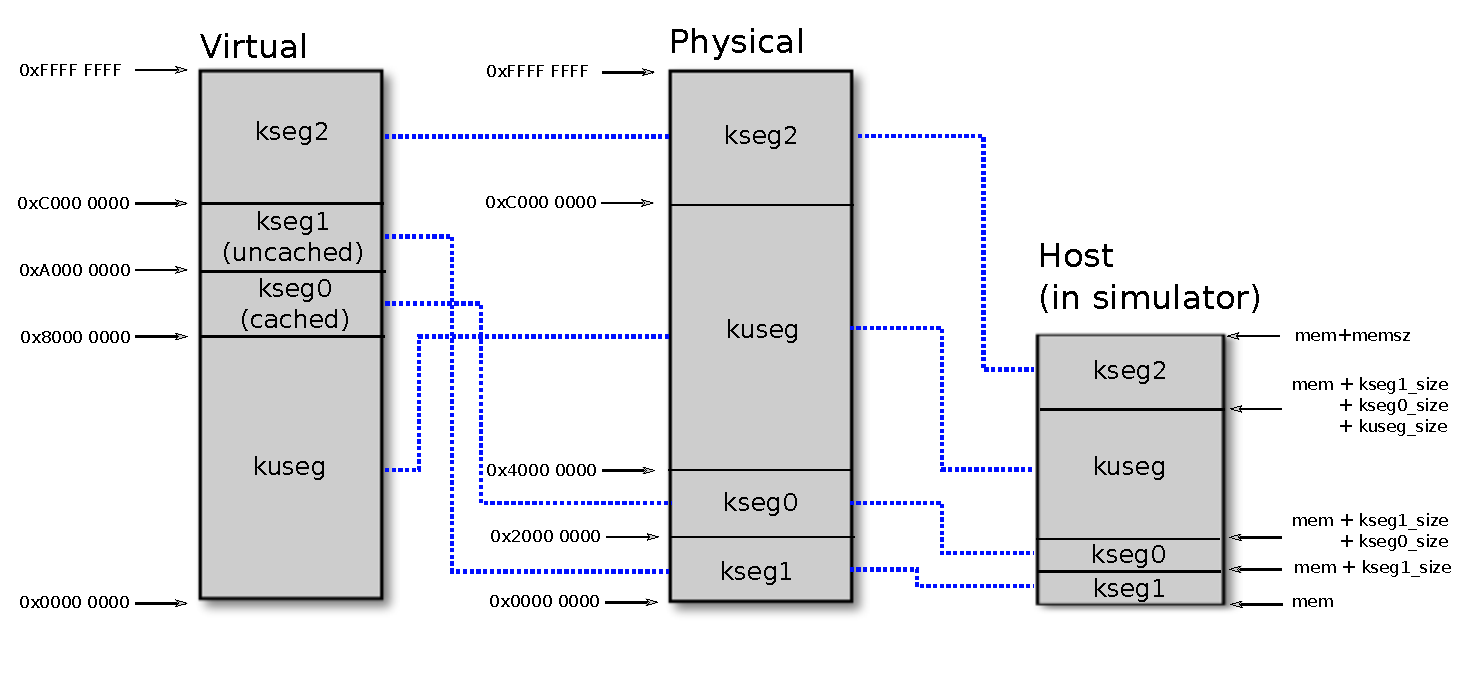
\includegraphics[width=\textwidth]{mmu/memory_mapping.eps}
	\caption{Main memory mapping in the simulator.}
	\label{fig:address_space_mapping}
\end{figure*}




\section{Memory Mapped IO}
\label{sec:io}
There are multiple ways a computer can communicate with its peripheral devices.
The most used techniques are Memory-Mapped I/O (MMIO) and Port-Mapped I/O
(PMIO). Port-Mapped I/O is an older method of accessing peripherals, and is much
more common in consumer computers with Intel or AMD CPUs\cite{intelmanual}.\\
PMIO requires the processor to have additional pins and special instructions,
just for communication with I/O devices. I/O devices have a specified port
number, which the processor uses to identify and communicate with the device,
much like an address.
For example, Intel x86 processors might be polling
%\footnote{Polling refers to the activity where a CPU periodically samples the status of an external device}
a keyboard using the special \texttt{in} instruction, specifying the predefined
keyboard status ID \texttt{0x60}, then reading from keyboard data, with ID
\texttt{0x64}\cite{intel:pch}\cite{osdev:io_ports}:
\begin{lstlisting}[language={[x86masm]Assembler}]
_wait:
  in  al, 64H ; Read keyboard status
  and al, 1   ; Check if ready
  jz  _wait
  in  al, 60H ; Read keyboard data
\end{lstlisting}
Besides the added circuitry in the processor, port-mapped I/O are fairly
simple to implement for chip manufacturers, and easy to use for programmers.
They have their own special instructions,
and they do not share memory space, which prevents confusion about
memory segmenting.
However, PMIO approach is very limited to only \texttt{in} and \texttt{out}
instructions, reading only a few bytes at a time into the EAX register, as well
as a limited number of ports for devices.\cite{intelmanual}\\

Memory-Mapped I/O is commonly used by RISC architectures. In MMIO,
communication with the peripherals happens over the same address bus as the
memory, so that memory and I/O communication share address space. This means
that when a processor, that uses MMIO, wants to access a peripheral, it uses a
memory address for communication.\\
The advantage of memory-mapped I/O is that the method uses already existing
memory bus lanes for communication, unlike the port implementation. However,
since the memory is shared with peripherals, and these addresses are not
maintained by the processor, additional logic has to be created in the
memory-management unit (discussed in the previous section).
%However, PMIO is very limited to the simple \texttt{in
%/ out} instructions, as well as a hardware-limited device allocation, whereas
%MMIO is much more free with device "address" allocation.

 Due to these reasons,
memory-mapped I/O is becoming increasingly popular, even on modern x86
hardware\cite{osdev:io_ports}.\\
MIPS initially sees Input/Output (IO) devices as a set of special-purpose registers. These
special registers are the processors only way of communicating with a given
device.\\
For every device, there 3 types of
registers\cite{cs_uwm:memory_mapped_io}\cite{imgtec:pra}:
\begin{itemize}
	\item \texttt{Status registers}\\
	Provide information about the underlying device. These registers are
	read-only for the CPU.

	\item \texttt{Control registers}\\
	Used to communicate and control the device. These registers are
	writeable by the CPU, but may not always be readable.

	\item \texttt{Data registers}\\
	Used for the actual data-transport. For example, the latest key pressed
	on the keyboard might be stored in a data register.
\end{itemize}

On MIPS32, these registers have allocated 4 memory bytes each, and are
always located sequentially in the memory.

For example, figure \ref{fig:io_registers} shows an example of IO register
layout of a very simple keyboard device.
\begin{figure}[H]
	\centering
	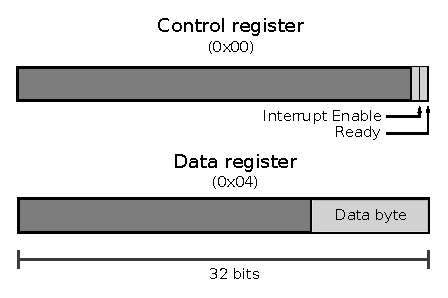
\includegraphics[scale=1]{io/io_registers.eps}
	\caption{Set of memory mapped I/O registers\cite{imgtec:pra}}
	\label{fig:io_registers}
\end{figure}

When a device is detected, the memory-management unit will allocate an address
for the device, notifying both the CPU and the device of these newly allocated registers.
From now on, it is up to the driver to interface with the devices.\\
Depending on the type of the IO device, the device can be represented from a
few registers to dozens. For example, a mouse or a keyboard only transmits few
bytes of information at a time, needing only a few registers, while graphic
adaptors or disk drives might need more\cite{cs_uwm:memory_mapped_io}.\\
These special-purpose registers are located in memory, mapped to a certain
segment. A device controller maintains a list of these registers, and maps new
devices to memory.\cite{britton:mips}\\
On MIPS32, the highest 64 kilobytes (\texttt{0xffff0000 - 0xffffffff}) in the
available memory are used for mapping these special registers\cite{cs_uwm:memory_mapped_io}.
The memory mapping of the IO area must not be cached, as a cache assumes the
memory is only modified from the CPU, and not by any external device, such as
an IO device.\\
However, it is obvious that IO registers can be very inconvenient for larger and
fast data-transfer, due to the very limited register size. To dodge this
bottleneck, memory controllers are implemented to give IO devices direct access
to larger parts of the main memory, without the need of going through the CPU first.

\subsection{Direct Memory Access}
Direct Memory Access controllers, also called DMA controllers, allow certain
hardware to access the main memory independently of the CPU.
In MIPS, this feature is built-in in the MMU.\\
Larger transfers between hardware and memory are usually initiated through
the device registers, where the CPU sets up the MMU and communicates the target
address. Then, the IO device is free to read and write in the target address.
When the peripheral is finished with its memory actions, it will usually
notify the CPU using an interrupt, having the processor taking care of the rest.\\
Direct Memory Access is often utilized by peripherals with heavy IO use, such
as the storage drives, as well as network-, sound-, and graphics-cards.\\
Because KUDOS does not read large portions of data from its IO devices, nor is
there any DMA support in the current YAMS simulator, DMA will not be implemented.

\subsection{Detecting and mapping peripherals}
When a computer is turned on, or a new peripheral device is plugged in, the MIPS
processor and its MMU automatically map the device to a given address, allocating
the necessary IO registers. All this happens seamlessly and without the interaction
of the operating system. This is problematic, because the OS needs to know the
type of the device and the address of its memory mapped registers, amongst other
things. There is no real way to communicate this between the processor and the
operating system. To make matters worse, each processor has its own addresses
for the registers, and a slightly different configuration. On top of that, each
board has its own set of external components, busses and metadevices\cite{devicetree_spec}\cite{xillybus:devicetree}.
Instead of compiling a very specialized kernel for seemingly every configuration
of a System on a Chip (SoC), operating system and bootloader developers have
designed a specification \emph{devicetree}, which is used to describe system
hardware\cite{devicetree_spec}.\\
The devicetree specification can describe a lot of aspects of a hardware devices,
such as the interrupt number, size of the IO registers, even the device clock
speeds.\\
The Linux kernel also enjoys this devicetree specification, both for ARM and
MIPS architecuters\cite[\texttt{linux-4.6/arch/mips/boot/dts}]{linux}, reducing the time
and complexity of implementing a new board or a SoC.\\
In KUDOS, this data structure is unfortunatelly not used, because the hardware
it runs on is very limited, consisting almost only of simulated devices. As
a result of that, KUDOS looks at a predefined address for data structures
describing the devices, called the device descriptors.

\subsection{Device descriptors}
To detect and communicate with external devices, device descriptors are used.
A device descriptor is a data structure which, just like a devicetree, specifies
all the relevant information about the device, such as its type, name, register
addresses and so on. The format of the device descriptor is defined in Yet Another
MIPS Simulator, the current simulator used to run KUDOS. The same device descriptor
structure is defined in KUDOS, so that KUDOS can interface with the underlying
simulator, retrieving the relevant information.
The structure is defined in \cite[kudos/drivers/mips32/arch.h]{kudos} as:
\begin{lstlisting}[language=c]
typedef struct {
    uint32_t type;
    uint32_t io_area_base;
    uint32_t io_area_len;
    uint32_t irq;
    char vendor_string[8];

   /* Reserved area (unused). */
    uint32_t resv[2];
} io_descriptor_t;
\end{lstlisting}

Learning from the devicetree specification and the seasoned Linux developers,
it would probably be better with a more general method to describe system
hardware. However, to be compatible with KUDOS and not break it, we will use
this exact same interface with devices, although modifying its location in
memory slightly.


\subsection{Implementation}
The OS, or rather, KUDOS in our case, needs to know the exact memory address of
the device descriptors, so that it can interact with the underlying IO devices.
KUDOS and the simulator agree on a memory address, which is the start of the
device descriptor area. In KUDOS and the simulator, this area is defined by
\texttt{IO\_DESCRIPTOR\_AREA}, with the value of \texttt{0xFFFE0000}. From there,
KUDOS searches for the underlying devices. The structure is represented on figure
\ref{fig:io_memory_layout}

\begin{figure}[H]
	\centering
	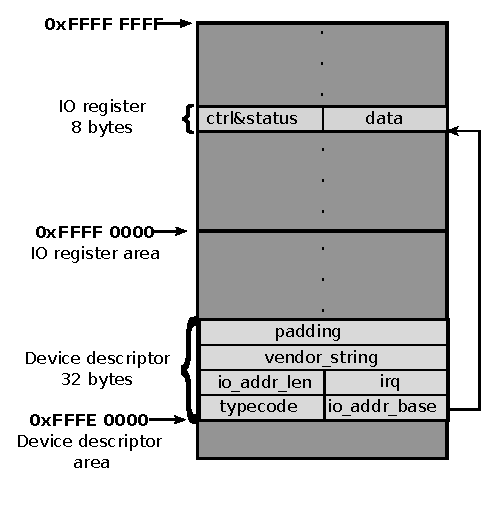
\includegraphics[scale=1]{io/io_memory_layout.eps}
	\caption{Memory layout of IO device descriptors and registers.}
	\label{fig:io_memory_layout}
\end{figure}

\subsection{Hardware Devices}
Naturally, we are going to need to implement some essential hardware devices
for KUDOS to use.\\
There are no definite specifications for how a hardware device must work.
Effectivelly, each manufacturer decides the specification of their devices
themselves. It is impossible for an operating system to keep track of all these
devices, and so, a special kind of interface, called a \texttt{driver},
is implemented and used for each device.\\
Most drivers are specific to certain devices, removing the subsequent complexity
for the communication with the device. This is also why certain devices refuse
to work in Linux, Windows or other OS, before the correct driver is installed
\cite{microsoft:driver}.\\
Lucky for us, we can define our own devices and its drivers -- that is,
we do not emulate an existing device, rather we define our own, with its own
set of magic numbers, IO registers etc.


\subsubsection{Shutdown device}
The first most important device is the shutdown-device, which powers off the
machine (in our case, the simulator).
In KUDOS and YAMS, this device is implemented with only 1 data register, which
will trigger a shutdown, if a magic number \texttt{POWEROFF\_SHUTDOWN\_MAGIC} is
written to it\cite[drivers/metadev.h]{kudos}.\\
In the simulator, if the write-address is that of the shutdown device, and the
magic number is known, the global boolean variable \texttt{g\_finished} is
toggled, stopping the simulator.\\
Once again, to avoid unneccesarry compatibility breaks with YAMS, we will use
the same magic number.

\subsubsection{TTY device}
To avoid a separated keyboard and display, a TTY device is implement, which
takes care of both. Once again, it will use the same number of IO registers
and the same typecode, so that the KUDOS TTY drivers do not have to be
re-written.\\
For usability, the TTY device needs to be controlled from a separate terminal
emulator, as
the simulator itself prints a lot of logging, debugging, and error messages,
which would choke the actual OS input and output.
For simplicity of the simulator, this TTY window will be implemented in a
separate program, which will wait for the simulator to start, and then connect
to it.\\

\subsubsection{External program communication}
Each external program, that acts as an IO device, needs a way
to communicate with our simulator. In Linux systems, there are multiple ways for
separate programs to communicate, such as using files, sockets, signals,
message passing as well as named pipes and shared memory\cite{love2013linux}.\\
For simplicity, the simulator and the programs will use shared memory model,
in which the OS will create and share a section of the process' memory,
identified with a key.\\
In the simulator, the IO register memory area will be split up into chunks of
shared memory, each identified with a unique key. Every IO device, that the
simulator supports, will have this key, and use it to access the registers at
the location.\\
Since MIPS32 does not implement interrupt numbers, we need not need any elaborate
way of signalling the counterpart program of an event -- we simply need a binary
signal, just as the one implemented in the bare-metal of the processor. Thus,
for signalling an interrupt, the simulator uses a POSIX user-defined signal
\texttt{SIGUSR1}, which will be our indicator of an event.\\
This way, the simulator and the device can work independently of each other.


\section{Tests}
It is essential to repeatedly perform tests on the simulator, to ensure its
correct behaviour, and in cases, detect and fix errors and other bugs.\\
To very first tests ensure the basic functionality of the simulator, usually
testing each instruction for the correct behaviour. When the simulator gets more
advanced, additional features are added, that also need to be tested.

\subsection{Basic tests}
Tests for the correct behaviour of an instruction is very simple. Each test uses
the related instruction in as many ways as possible, using as few other
instructions as possible. For example, the \texttt{add} instruction is tested
for both being able to add, but also subtract in one test.\\
For simplicity, the tests return their value in \texttt{\$v1}, which the
simulator uses as its exit value.\\
All test programs lie in the \texttt{tests/} subdirectory, with a corresponding
file ending with \texttt{".text"}, containing the expected result.
To run all tests, a bash script \texttt{run\_tests.sh} is stored on the project
root, which runs each test program with the simulator, comparing the return
value with the expected return value.

\subsection{Advanced tests}
Executing instructions is only a part of the simulation. The simulator also
needs to be able to handle certain situations and problems correctly, and
according to the specification.\\
One of these advanced tests is the pipeline testing, which are programs
with instructions structured in a way so that the pipeline forwarding unit and
hazard unit are used repeatedly. If one of these units fail, the result will be
seen immediately on the output value.\\
Other more advanced tests ensure many side-effects of instructions, such as the
branch-delay slot, or correct flag-toggling of the status register on exception
occurrence.

\subsection{Travis-CI}
TO BE WRITTEN

\subsection{Partial conclusion}
Having a suite of testing programs for each instruction was a tremendous help to
find and fix bugs.\\
However, a big issue with the test suite is that some of the tests depend on
other instructions to work, as to setup the test. This is not necessarily
always the case, and can cause false-negatives, or worse, false-positives.
Optimally, the simulator should be able to start in a certain state, defined by
some configuration file, describing the values and flags of all the processor
registers, flags, even pipeline registers. This would help to test certain
cases in the simulator, avoiding possible side-effects of other possibly faulty
instructions.\\
Another small, but useful improvement would be having dynamic tests, that would
generate test values on every run, so that each time a test is run, it uses new
values, covering a bigger area of the instruction, and further increasing the
chance of finding a bug in the simulator.


\section{Performance}
Although the primary objective of the simulator is not the performance, it is
an interesting aspect to study.\\
The pipeline approach of the simulator takes a lot of processing to perform,
and is implemented only for academic purposes -- to study the state and behaviour
of the processor. It goes without saying that the pipeline is not needed to
emulate the target CPU, as the emulated instructions are not held back by a time
restricting clock, nor do they have to wait for result from the previous instruction to
continue.\\

\subsection{Comparison}
The simulator is compared to its predecessor YAMS using GNU debugger (GDB). GNU debugger
is a program used to debug, control and inspect other programs. It is a widely
used and very powerful tool used for development on Linux\cite{gdb}.\\
In GDB, a breakpoint is set on every simulator clock tick, that is, every time
the simulator reaches to the start cycle of simulating a new instruction. Then,
GDB steps to next instructions, until the breakpoint is reached again. This
process is repeated a number of times, the number of "steps" saved and printed
at the end. A GDB script \texttt{perf.gdb} is used for this task, which consists
of two \texttt{while} loops - one iterating over the number of simulated instructions,
and the other one counting the host instructions used. At the end of the script,
GDB prints \texttt{\$i}, which is the number of simulated instructions executed,
and \texttt{\$count}, which is the number of host instructions used. The script
can be seen on figure \ref{fig:gdb_perf}.
\begin{figure}
\lstinputlisting[caption=]{../perf.gdb}
\caption{GDB script to test performance.}
\label{fig:gdb_perf}
\end{figure}

Due to compatibility, the simulator will executing KUDOS, while YAMS will be
executing BUENOS. Although this might cause the simulators to execute different
instructions, the test runs enough instructions to approximate their performance.

\begin{center}
    \begin{tabular}{ | c | c | c | c | r | }
    \hline
    & i = 10 & i = 1000 & ratio \\ \hline \hline
    \texttt{YAMS} & 3545 & 430328 &  429\\ \hline
    \texttt{Simulator} & 9218 & 788851 & 790 \\ \hline
    \end{tabular}
\end{center}

%
%CKUDOS RUn
%\$1 = 92183
%\$2 = 10
%
%\$1 = 788851
%\$2 = 1000
%
%
%YAMS
%\$1 = 3545
%\$2 = 10
%
%\$3 = 430328
%\$4 = 1000

By this very primitive test, YAMS is approximatelly 2 times faster, as it uses
the half the instructions to emulate an instruction.\\
On the testing computer, an Intel® Core™ i5-6200U Processor is used, with turbo
frequency up to 2.80GHz\cite{intel:i5}. If fully utilized, the simulator can on
this machine simulate a very fast MIPS processor with over 3.5MHz clock rate,
which is more than enough for the KUDOS operating system:
$$\frac{2.80\mathit{ GHz}}{790} \approx 3.5443\mathit{ MHz}$$
As the YAMS simulator runs at default 1 MHz\cite{yams}, the speed of 3.5 MHz yields enough
room for improvements and additional systems to be implemented in the simulator.


\section{Running KUDOS}
The simulators main target is to run KUDOS, and so, operating systems such as KUDOS
can be run just as any other userspace program.\\
For initial testing purposes, KUDOS is modified to startup, initialize only
the shutdown device, and trigger the shutdown device.\\
When running the simulator (git commit version \texttt{0ff2a1c8}) on the modified
KUDOS, a crash occurs:
\begin{verbatim}
$ bin/mips-sim -l out.txt kudos-mips32
...
[ERROR] src/mem.c, translate_paddr():216:
ADDRESS OVERFLOW, PADDR: 0x40000004.
Out of bounds: 0x38000000
Segmentation fault (core dumped)
\end{verbatim}
Inspecting the code, the crash occurs at \texttt{0x80011034}\footnote{The instructions
are logged when they enter the pipeline, but the instruction causing the fault is
in memory stage.}. Since KUDOS correctly only uses the user segment (\texttt{kuseg})
for user-space programs, the modified version of KUDOS, which does not start
any userspace programs, should \textit{never} write to the middle of the user segment.\\
The faulting instruction address is located just at the start of \texttt{semaphore\_P},
which are not used in the modified KUDOS. Indeed, the simulator has gone wild and
continued execution, where it should clearly have been shutdown, until a crash
occurs.\\
Upon further inspection of the code, a very peculiar behaviour is uncovered ---
the simulator enters a kind of "NOP" sled, that is, a long section of a program
that only consists of instructions that do nothing. This occurs after instruction
located at \texttt{0x80000084}:
\begin{verbatim}
0x8001891C: 0x1466FFFA  BNE  rs = ...
0x80000088: 0x00000000  SLL  rs = ...
0x8000008C: 0x00000000  SLL  rs = ...
0x80000090: 0x00000000  SLL  rs = ...
0x80000094: 0x00000000  SLL  rs = ...
0x80000098: 0x00000000  SLL  rs = ...
0x8000009C: 0x00000000  SLL  rs = ...
\end{verbatim}
Another peculiar behaviour is exposed --- the program executes in kernel segment
(\texttt{> 0x80000000}), but it is not after the KUDOS start-point \texttt{0x80001000}.
However, the instruction prior can be tracked down to be the comparison of the
device typecode of the shutdown function:
\begin{verbatim}
8001891c: bne v1,a2,80018908 <shutdown+0x34>
\end{verbatim}

It is clear that the execution can not continue at the "NOP-sled" addresses,
and therefore, a bug is present in the address translation mechanism in the simulator,
more specifically, the \texttt{translate\_paddr(...)} function of the memory module.


\section{Conclusion}
The simulator has been written using modules resembling the actual design of
MIPS32 processors. This yields a natural flow of instructions, as well as a very natural
behaviour of the actual code.\\
While the simulator can successfully run all the test-cases supplied along side
the code, we have shown that the simulator still contains bugs that, when running
KUDOS, will cause the simulator to continue execution at unknown memory addresses,
eventually reaching some actual code that will make the simulator enter an invalid
state, and crashing. However, despite this bug, enough material has been presented
to show that a pipelined MIPS32 simulator with a working MMU, memory-mapped IO,
exception mechanism as well as debugging functions, can be written, with excellent
performance. After comparison to the more field-tested YAMS, the simulator was
only about half as fast, with all the same features as its counterpart. However,
due to the low performance requirements of the KUDOS system, the simulator should
be more than fast enough.




\newpage
\clearpage % force new page(?)
\bibliography{mybib}{}
\bibliographystyle{plain}

\newpage
\appendix
%\begin{appendices}
% Appendix here
%\end{appendices}

\end{document}
